\documentclass{article}

\usepackage[utf8x]{inputenc}
\usepackage[english,russian]{babel}
\usepackage{cmap}
\usepackage{commath}
\usepackage{amsmath}
\usepackage{amsfonts}
\usepackage{mathtools}
\usepackage{amssymb}
\usepackage{parskip}
\usepackage{titling}
\usepackage{color}
\usepackage{hyperref}
\usepackage{cancel}
\usepackage{enumerate}
\usepackage{multicol}
\usepackage{graphicx}
\usepackage[font=small,labelfont=bf]{caption}
\usepackage[a4paper, left=2.5cm, right=1.5cm, top=2.5cm, bottom=2.5cm]{geometry}

\graphicspath{ {./images/} }
\setlength{\droptitle}{-3cm}
\hypersetup{ colorlinks=true, linktoc=all, linkcolor=blue }
\pagenumbering{arabic}

\begin{document}
    \textbf{Теорема 1.} Пусть $f:\ A \rightarrow A$ вложение, и множество $A$ содержит конечное число элементов. Тогда отображение $f$ --- биекция.
    
    $\uparrow$ Надо показать, что $f$ --- наложение, т.е. каждый элемент $a \in A$ имеет прообраз $a':\ a = f(a')$. Обозначим $\underbrace{f \circ f \circ ... \circ f}_{k} = f^k$. В силу конечности множества $A$ в последовательности элементов $a, f(a), f^2(a), ...,$\\ $f^m(a), ..., f^n(a), ...$ должны быть повторения.
    
    Предположим, что
    \[f^m(a) = f^n(a) \text{ и } m < n.\]
    Если $m > 0$, то $f(f^{m - 1}(a)) = f(f^{n - 1}(a))$, и поскольку $f$ --- вложение, то $f^{m - 1}(a) = f^{n - 1}(a)$.

    Продолжим процедуру ``сокращения`` пока не придем к соотношению
    \[a = f^{n - m}(a) = f(f^{n - m - 1}(a)).\]
    Искомым элементом $a'$ оказался $f^{n - m - 1}(a): a = f(a')$. $\downarrow$

    \textbf{Определение 11.} Тождественным (или единичным) отображением множества $A$ на себя назовем отображение $I_A$, оставляющее неизменным все элементы из $A$:
    \[I_A:\ x \rightarrow x,\ \forall\ x \in A.\]

    \textbf{Свойство.} Ясно, что $f \circ I_A = f,\ I_B \circ f = f$.

    \textbf{Теорема 2.} Отображение $f: A \rightarrow B$ является биекцией тогда и только тогда, когда найдется такое отображение $g:\ B \rightarrow A$, что $g \circ f = I_A$ и $f \circ g = I_B$.
    
    $\uparrow$ ``$\Rightarrow$`` Пусть $f$ является биекцией. Тогда всякий $y \in B$ имеет прообраз $x \in A$ (так как $f$ --- наложение) и притом единственный (так как $f$ --- вложение). Это позволяет определить отображение, переводящее $y$ в свой единственный прообраз $x$. Естественно обозначить это отображение символом $f^{-1}$ и назвать обратным отображением.
    
    \textbf{Определение 12.} Отображение $f^{-1}: B \rightarrow A$ называется обратным отображением к отображению $f:\ A \rightarrow B$, если оно переводит каждый элемент $y \in B$ в свой единственный прообраз $x \in A$. $f^{-1}:\ y \rightarrow x = f^{-1}(y)$.
    
    Так как $y = f(x)$, то $x = f^{-1}(y) = f^{-1}(f(x)) = f^{-1} \circ f(x)$, и $f^{-1} \circ f = I_A$.
    
    С другой стороны, $y = f(x) = f(f^{-1}(y)) = f \circ f^{-1}(y)$, и $f \circ f^{-1} = I_B$.
    
    Т.е. роль $g$ играет $f^{-1}$.

    ``$\Leftarrow$`` Доказательство обратного утверждения разобьем на два этапа:

    1) Имеем $g \circ f = I_A$. Покажем, что $f$ --- вложение. Пусть $x_1$, $x_2 \in A$ и $x_1 \neq x_2$. Надо показать, что $f(x_1) \neq f(x_2)$. Так как $x_1 = I_A(x_1) = g(f(x_1)),\ x_2 = I_A(x_2) = g(f(x_2))$, то по предположению $g(f(x_1)) \neq g(f(x_2))$. Но тогда и $f(x_1) \neq f(x_2)$, так как от противного: если $f(x_1) = f(x_2)$, то и $g(f(x_1)) = g(f(x_2))$, так как $g$ --- отображение и каждому элементу ставит в соответствие ровно один элемент (противоречие).

    2) Имеем $f \circ g = I_B$. Покажем, что $f$ --- наложение. Надо $\forall\ y \in B$ имеет прообраз.\\
    Так как $y = I_B(y) = f(g(y))$, то в качестве прообраза выступает $x = g(y)$.\\
    Из 1) и 2) $f$ --- биекция. $\downarrow$
    
    \textbf{Замечание.} Отображение $g$, удовлетворяющее соотношениям $g \circ f = I_A$ и $f \circ g = I_B$, совпадает с обратным отображением $f^{-1}$.\\
    $\uparrow$ $g = I_A \circ g = (f^{-1} \circ f) \circ g = f^{-1} \circ (f \circ g) = f^{-1} \circ I_B = f^{-1}$. $\downarrow$\\
    Т.е. теорему 2 можно сформулировать и в терминах обратного отображения.

    \textbf{Теорема 2'}. Отображение $f:\ A \rightarrow B$ обладает обратным отображением тогда и только тогда, когда $f$ --- биекция.
    
    \textbf{Следствие 1.} Если $f$ --- биекция, то $f^{-1}$ тоже биекция.

    $\uparrow$ По Теореме $2$, $2'$ если $f$ --- биекция, то $\exists\ g = f^{-1}$ такое, что $f^{-1} \circ f = I_A$ и $f \circ f^{-1} = I_B$.\\
    Таким образом для отображения $f^{-1}$ существует такое $g' = f$, что выполнены условия теоремы $2$, и значит по доказанному (``$\Leftarrow$``) $f^{-1}$ тоже биекция и $(f^{-1})^{-1} = f$. $\downarrow$

    \textbf{Следствие 2.} Пусть $f:\ A \rightarrow B$ и $h:\ B \rightarrow C$ --- биекции. Тогда $h \circ f:\ A \rightarrow C$ --- биекция.
    
    $\uparrow$ Рассмотрим отображение $f^{-1} \circ h^{-1}$.

    $(f^{-1} \circ h^{-1}) \circ (h \circ f) = f^{-1} \circ (h^{-1} \circ h) \circ f = f^{-1} \circ I_B \circ f = f^{-1} \circ f = I_A$;

    $(h \circ f) \circ (f^{-1} \circ h^{-1}) = h \circ (f \circ f^{-1}) \circ h^{-1} = h \circ I_B \circ h^{-1} = h \circ h^{-1} = I_C$.

    Тогда в силу Теоремы $2$, $h \circ f$ --- биекция и $(h \circ f)^{-1} = f^{-1} \circ h^{-1}$. $\downarrow$

    \section{Функции и графики}

    \textbf{Уточнение.} Отображение, действующее из числового множества в числовое множество, принято называть функцией.
    
    Ещё раз поговорим о способах задания функций.

    \textbf{1. Формульное задание.} $y = f(x)$, где $f(x)$ --- аналитическое (формульное) выражение. Это самый распространенный и точный способ.

    \textbf{Пример.} $y = x^2,\ y = \begin{cases}
        \sqrt{1 + x^2}, & x > 0\\
        0, & x = 0\\
        -\sqrt{1 + x^2}, & x < 0\\
    \end{cases}$

    При формульном задании удобно говорить о естественной области определения, т.е. о множестве тех $x \in \mathbb{R}$, при которых выражение $f(x)$ имеет смысл. Так $y = 1− x$ определена при $x \leq 1$, $y = \frac{1}{x}$ при $x \in \mathbb{R} \backslash \{0\}$. Однако, из каких-либо соображений функция может быть задана (или рассмотрена) и на некотором другом множестве: $y = \frac{1}{x}$ при $x \in [1, 2]$. Функции $y = \frac{1}{x}$ при $x \in \mathbb{R} \backslash \{0\}$ и $y = \frac{1}{x}$ при $x \in [1, 2]$ различны, отличаются множества, на которых они рассматриваются ($A$).

    В качестве области значений можно взять всё $\mathbb{R}$ или в точности образ $A$ при отображении $f:\ f(A)$.

    \textbf{Пример.} Найдите область определения и область значений функции $y = \sqrt{8x - x^2 - 12}$.

    Найдем $A = D_f$. Рассмотрим функцию $y_1 = -x^2 + 8x - 12 = -(x - 2)(x - 6)$. Решая неравенство $y_1 \geq 0$, получаем $x \in [2, 6]$.

    Найдем $B = f(A) = E_f$. График функции $y_1$ --- парабола, ветви которой направлены вниз. Наибольшее значение эта функция принимает при $x = 4$ (вершина параболы). Поэтому на промежутке $x \in [2, 6]$ функция $y_1$ принимает значения от нуля до $y_1(4) = -16 + 32 - 12 = 4$. Т.е. $y_1 \in [0, 4]$. Функция $\sqrt{}$ --- монотонно возрастающая функция, поэтому $E_f = [0, 2]$.
    
    \textbf{2. Алгоритмическое (описательное или словесное) задание.} Указано четкое правило, по которому каждому $x \in A$ ставится в соответствие $y \in B$.
    
    \textbf{Пример.} $y(x) = min(10 \textrm{ и } 9 \textrm{ цифры в десятичной записи числа } x)$.

    \textbf{3. Табличное задание функции.} Понятно, что если функция $f$ задана на бесконечном множестве точек, например на отрезке, то таблицей её задать нельзя. Однако, если таблица --- результат экспериментальных данных, то можно аппроксимировать (приблизить) функцию во всех внутренних точках. Аппроксимацию можно проводить различными способами. Сейчас есть программы, с помощью которых, задав множества $(x_1, x_2, ..., x_n)$, $(y_1, y_2, ..., y_n)$ и примерный вид функции (например, $y = a_{k}x^{k} + a_{k - 1}x^{k - 1} + ... + a_{0},\ y = a\ sin\ bx * e^{cx}$ и т.п), можно получить значения неизвестных коэффициентов $a_k, a_{k-1}, ..., a_0, a, b, c$ с наперед заданной точностью.
    
    \textbf{4. Неявное задание функции.} $F(x, y) = 0$. Т.е функция является решением некоторого уравнения (возможно дифференциального или интегрального). Иногда из этого уравнения можно выразить $y$ через $x$, т.е. перейти к заданию функции формулой, но далеко не всегда! Вообще говоря, уравнению $F(x, y) = 0$ может удовлетворять не одна функция, а множество функций.
 
    \textbf{Пример.} $x^2 + y^2 = 1$. Уравнению окружности удовлетворяют две функции: $y_1 = \sqrt{1 - x^2}$ и $y_2 = -\sqrt{1 - x^2}$.
    
    % \begin{figure}[h!]
    % \centering
    % 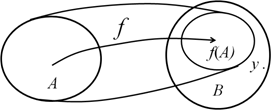
\includegraphics{2}
    % \caption{\label{fig:fig2}Разность и симметрическая разность множеств.}
    % \end{figure}

\end{document}